\documentclass[12pt, titlepage]{article}

\usepackage{booktabs}
\usepackage{tabularx}
\usepackage{hyperref}
\hypersetup{
    colorlinks,
    citecolor=black,
    filecolor=black,
    linkcolor=red,
    urlcolor=blue
}
\usepackage[round]{natbib}
\usepackage{enumitem}
\usepackage{graphicx}

\setlist[description]{leftmargin=\parindent,labelindent=\parindent}

\graphicspath{ {testResults/} }

\title{SE 3XA3: Test Report\\Password Protection ProgramG}

\author{Team 28, Team Name
		\\ Suhavi Sandhu sandhs11
		\\ Shabana Dhayananth dhayanas
		\\ Joseph Lu luy89
}

\date{\today}

\begin{document}

\maketitle

\pagenumbering{roman}
\tableofcontents
\listoftables
\listoffigures

\begin{table}[bp]
\caption{\bf Revision History}
\begin{tabularx}{\textwidth}{p{3cm}p{2cm}X}
\toprule {\bf Date} & {\bf Version} & {\bf Notes}\\
\midrule
Date 1 & 1.0 & Notes\\
Date 2 & 1.1 & Notes\\
\bottomrule
\end{tabularx}
\end{table}

\newpage

\pagenumbering{arabic}

This document discusses the results from testing the product, PasswordProtectionProgram, any changes that were implemented as a result of testing and the extensiveness of the tests performed.

\section{Functional Requirements Evaluation}

	\subsection{User Input}
	
		\subsubsection{Master Password}
			These test cases verify that the functions related to the master password, a critical part of the system, behave as intended.\\
			
			The following test cases assume that a master password has not yet been initialized and test for the creation of the master password.
			
			\begin{itemize}
			
				\item \textbf{FR-MP-1}: A valid input of at least characters having upper and lowercase as well as numbers should let user proceed.\\
				 Result: Test pass, user is allowed to proceed.
				 
				\item \textbf{FR-MP-2} to \textbf{FR-MP-5}: Invalid input for master password should display appropriate error message.\\
				 Results: All tests pass and display appropriate error message.
			
			\end{itemize}
			 
			The following test cases assume that a master password has already been initialized and test for logging in with the master password.\\
			
			\begin{itemize}	 
			
				\item \textbf{FR-MP-6}: Upon entry of an empty string, the system should display an error message.\\
				Result: This test originally passed, however, due to a bug found during the testing for ‘update entry’, this test was omitted.
				
				\item \textbf{FR-MP-7}, \textbf{FR-MP-8}: Depending on whether input is correct or incorrect, system lets user proceed or displays error message.\\
				Result: Tests pass
			
			\end{itemize}

		\subsubsection{Adding Entries}
			These tests verify that users are able to add new entries to the database, assuming a connection to the database is already established and user is logged into application.\\

			\begin{itemize}	

				\item \textbf{FR-AE-1}, \textbf{FR-AE-2}, \textbf{FR-AE-3}: Originally, the goal of these test cases was to ensure that when adding an entry, a user cannot add an empty password. Upon testing, it became clear that an empty password should be allowed, in the case that the user has not come up with one. Therefore, the test was changed to verify that a Name, rather than a password, should be required.\\
				Results: All test cases pass, allowing users to add entries as long as name is provided, else error message displayed. 

			\end{itemize}

	\subsection{Navigation}
		The underlying goal for the product was to make it more userfriendly than the original. In doing so, great care was given to the tests designated under navigation. The following tests verify the functionality of the user manual.\\
		
		\begin{itemize}	

			\item \textbf{FR-N-1}: Link to user manual works.\\
			Results: A pdf viewer opens up with the user guide.
			
			\item \textbf{FR-N-2}: At view entry screen, clicking the question mark should take user to instructions page\\
			Results: Test passes, proving that  instructions are readily accessible.

			\item \textbf{FR-N-5}: User should be able to copy a password or username that is in the system database.\\
			Results: Copy button works as intended, test passes
			
			\item \textbf{FR-N-6}, \textbf{FR-N-7}: test the functionality of the generate button and verify that a string is outputted and can be called random through visual inspection.\\
			Results: All tests pass, output is random to the eye.

			\item \textbf{FR-N-8}: Tests the delete button, ensuring that all entries can be deleted, except master password.\\
			Results: Test passes, deleted entries are immediately removed and the database as well as the interface reflects these changes.

			\item \textbf{FR-N-9}: Tests the update button, ensuring that all entries’ password and usernames can be changed.\\
			Results: Test passes.\\
			\textbf{Further discussion}: This test led to the discovery of a bug that results from updating a master password to be an empty string. It is a legal action, however, when the user attempts to log back in with the updated password, he/she is prohibited since an empty string was not allowed. A temporary workaround for this bug is to allow empty strings but in the future, there will be unique constraints for updating passwords (i.e cannot be empty).

		\end{itemize}

	\subsection{Encryption}
		
		\begin{itemize}
			
			\item \textbf{FR-E-1}, \textbf{FR-E-2}: Check that a string being encrypted can ultimately be decrypted to give the original.\\
			Results: All tests pass.
		
		\end{itemize}	

	\subsection{Database}
		These tests have to do with the functionality of the database and ensure that it works independently to the rest of the system. Therefore, it is vital to ensure basic methods such as insert, delete, and update work as intended - something that can be proven with the test cases mentioned below.

		\begin{itemize}
			
			\item \textbf{FR-DB-1}: Database can be created
			\item \textbf{FR-DB-2}: Database has already been created
			\item \textbf{FR-DB-3}, \textbf{FR-DB-4}: When multiple entries exist, database should delete them when user deletes and return them when needed:\\
			Results: All tests pass. 

			
		\end{itemize}

	\subsection{Password Generation}

		\begin{itemize}

			\item \textbf{FR-PWG-1}: This test case ensures that the criteria for what the team defined as random is achieved by the method.\\
			Results: Test passes. It can be proven that the method generates passwords with exactly 8 characters, including uppercase, lowercase and numbers.

		\end{itemize}

\section{Nonfunctional Requirements Evaluation}

	\subsection{Look and Feel Requirements}		
		The following requirements check that the application has a standard interface that is aesthetically pleasing. An example test case below describes generally what was evaluated.

		\begin{itemize}
		
			\item \textbf{NFR-LFR-1}: The user should be able to navigate between screens seamlessly through the use of available buttons. \\
			Results: This test case, like all others in the Look and Feel category, were performed manually by our peers. To ensure that the cases passed, a rating from 1 to 10 is provided from user.\\
			For all the tests the average scores were reasonable. 

		\end{itemize}

	\subsection{Personalization}

		\begin{itemize}

			\item \textbf{NFR-PSR-1}: The user should be able to specify the category for which they are adding an entry for. \\
			Results: This test was performed manually by peers, who gave feedback in the form of their experience with the personalization aspect as well as a number from 1-10 defining how customizable they felt the application was. In this category, the application received a 7 as the option to add categories is available although there is no sorting by category, something we wish to implement in the future.


		\end{itemize}

	\subsection{Understandability and Politeness Requirements}

		\begin{itemize}

			\item \textbf{NFR-UPR-1}: To better understand the needs of users, a survey was conducted in the form of informal interviews with peers that may be interested in using a password manager.\\
			Results: The outcome of the interview gave insight on the topic of intuitive interfaces. We learned that users are more likely to understand from visual cues rather than text-based as they are more universal. Hence, image symbols were used for as many buttons as possible.

		\end{itemize}

	\subsection{Performance}

		\begin{itemize}

			\item \textbf{NFR-PER-1}: To verify the performance of the system, processing time of the reset\_timer function, a function of the graphical user interface that keeps track of inactivity period, was determined and compared against a PROCESSING\_TIME = 1 second\\
			Result: The test passed, giving a processing time less than PROCESSING\_TIME, verifying that the performance is up to par with standards.

			\item \textbf{NFR-PER-2}: To verify that error messages are displayed within ERROR\_TIME, the function for checking an invalid password was timed.\\
			Result: The test passed, giving an error time less than ERROR\_TIME, again, proving that performance is sufficient.

		\end{itemize}

	\subsection{Operational and Environmnetal Requirements}
		The following requirement checks that the application is able to run with Linux and OSX.

		\begin{itemize}
			
			\item \textbf{NFR-OER-1}: The user should be able to run the application with the same functionality as if they are on Windows.\\
			Result: All funcationality tests passes on other operating systesms. 

		\end{itemize}

	\subsection{Security}
		As the application that we developed being a security applicaiton, testing for security is a high priority of the team.
	
		\begin{itemize}
			
			\item \textbf{NFR-SR-1}: When the user is creating a new password when starting the application for the first time. They must create the password within the Criteria of set, or the database will not take the password.\\
			Result: The test Passes. When entering insufficiently secure passwords, the user can not keep going.

			\item \textbf{NFR-SR-3}: When the application is left inactive for the allocated time given, the application logs out.\\
			Result: The test pass.

		\end{itemize}
	
\section{Comparison to Existing Implementation}	

	Apart from the coding language and narrowed scope, the PasswordProtectionProgram was not too different from the original implementation, Padlock. By executing manual tests on both implementations, it can be verified that the PasswordProtectionProgram successfully fulfils a majority of the main functions that were in the original implementation. Below are the results from those tests.\\
	
	Functional Tests\\

	\quad User Input

	\begin{itemize}
	
		\item \textbf{FR-MP-1} Creation of master password - can be performed successfully on both with ease. Original implementation, however, does not have criteria for master password (it can be a single character if desired)
		\item \textbf{FR-FR-MP-5} Empty string for master password creation - displays error message in both implementations
		\item \textbf{FR-FR-MP-7} Log in with master password - returning users can successfully login with correct master password
		\item \textbf{FR-FR-MP-8} Login with incorrect master password - both implementations display error message.
		\item \textbf{FR-FR-AE-1} Add an entry for account with name, type, username and password - Same categories are present for this and the original implementation however, duplicates are allowed in the original, something we disallowed to give users a better experience
	
	\end{itemize}
	
	\quad Navigation

	\begin{itemize}

		\item \textbf{FR-N-5} Copy password from existing entry - both implementations give users an easy way to access their passwords if they are too complex, by simply copying to clipboard
		\item \textbf{FR-N-6} Generate random password for account entry - both implementations have a generate button to give users the opportunity to have more complex usernames and passwords, though, both implementations have different criteria for generation (8 characters, numbers, etc)

	\end{itemize}
	
	Nonfunctional Tests\\

	\quad Operational and Environmental Requirements

	\begin{itemize}
		
		\item \textbf{NFR-OER-1} Compatibility with Windows, OSX, Linux OS - both implementations should ideally work on all 3 platforms and they did however, we did not get a chance to test the same for our executable
	
	\end{itemize}

	\quad Personalization

	\begin{itemize}

		\item \textbf{NFR-PSR-1} User can categorize usernames and passwords based on account type - this test failed for the PasswordProtectionProgram as there is no categorization by account type as of now. It may be implemented in the future so users can sort account data by category, similar to the original implementation

	\end{itemize}

	\quad Security
	
	\begin{itemize}

		\item \textbf{NFR-SR-3} Logs user out after 1 minute of inactivity - currently changed to 30 seconds for testing purposes, both implementations timeout after a minute.

	\end{itemize}	



\section{Unit Testing and Automated Testing}

	PyUnit was used to perform unit testing on the system. All of these tests were automated.\\

	Below is description of each test module and a trace of what test cases were tested in each test module.

	\subsection{\texttt{testCopy.py}}

		Tests \texttt{copy.py} by checking that the copy function accurately copies what is on the user’s clipboard\\
		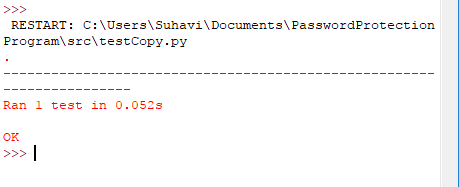
\includegraphics[scale=1]{testCopy.png}

	\subsection{\texttt{testDatabase.py}} 

		Tests \texttt{database.py} by checking that the main functions of the database such as insert, delete and update behave as intended

		\begin{itemize}		
			\item Tests \textbf{FR-DB-1}, add master password to empty database
			\item Tests \textbf{FR-DB-2}, update entry in populated database
			\item Tests \textbf{FR-DB-3}, delete entry in populated database
			\item Tests \textbf{FR-DB-4}, return all information in populated database
		\end{itemize}
		
		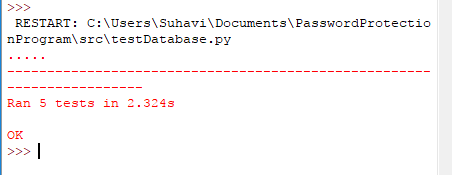
\includegraphics[scale=1]{testDatabase.png}

	\subsection{\texttt{testEncrypt.py}}
	
		Tests \texttt{Encrypt.py} by checking that key generation, encryption and decryption work

		\begin{itemize}
			\item Tests \textbf{FR-E-1}, encrypt strings
			\item Tests \textbf{FR-E-2}, decrypt an encrypted string
		\end{itemize}

		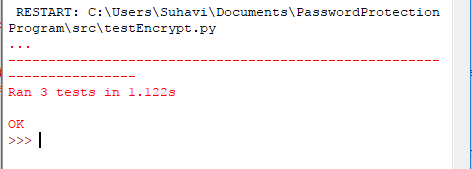
\includegraphics[scale=1]{testEncrypt.png}

	\subsection{\texttt{testGenPassword.py}}

		Tests \texttt{GenPassword.py} by checking that the random strings for username and password meet criteria

		\begin{itemize}
			\item Tests \textbf{FR-PWG-1}, criteria for random string generation (8 characters, upper,lowercase, number)
		\end{itemize}

		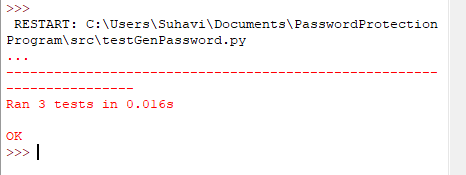
\includegraphics[scale=1]{testGenPassword.png}

	\subsection{\texttt{testPWChecking.py}}
	
		Tests \texttt{PWChecking.py} to verify that valid and invalid master password entries are handled correctly

		\begin{itemize}
			\item Tests \textbf{FR-MP-1} - create master password, following criteria (allowed)
			\item Tests \textbf{FR-MP-2} - create master password with no numbers (display error message)
			\item Tests \textbf{FR-MP-3} - create master password not at least 8 characters (display error message)
			\item Tests \textbf{FR-MP-4} - create master password with no uppercase (display error message)
			\item Tests \textbf{FR-MP-5} - create master password with empty string (displays error message)
			\item Tests \textbf{FR-MP-6} - later omitted 
			\item Tests \textbf{FR-MP-7} - login with correct master password (allowed)
			\item Tests \textbf{FR-MP-8} - login with incorrect master password  (displays error message)
		\end{itemize}

		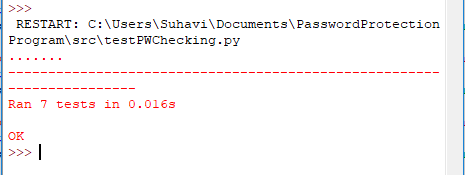
\includegraphics[scale=1]{testPWChecking.png}

	\subsection{\texttt{testResponseTime.py}}

		Tests \texttt{PPP.py} for its performance by checking PROCESSING\_TIME and ERROR\_TIME

		\begin{itemize}
			\item Tests \textbf{NFR-PER-1} - perform action within PROCESSING\_TIME
			\item Tests \textbf{NFR-PER-2} - display error message within ERROR\_TIME
		\end{itemize}

		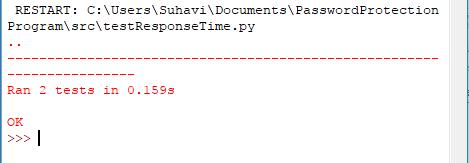
\includegraphics[scale=1]{testResponseTime.png}

\section{Changes Due to Testing}
	
	There were several changes that were implemented as a result of testing. These changes will be categorized by the main functional requirement that was affected.
	
	\begin{enumerate}

		\item \textbf{FR9} User should be able to change master password:\\
		While manually testing the update master password function, it was noticed that the master password could be updated to be an empty string, which is contradictory to the creation stage where the master password has to be at least 8 characters. As described earlier in the document, a change was made to the password checking module that accepts an empty string.
	
		\item \textbf{FR5} User should be able to add entries to the database\\
		While testing the adding entry function through integration of the interface and database, when the entries reached beyond the scrollbar, the scrollbar would not update to increase in size. To fix this, there was code added to refresh the application each time an entry is added. This made it less static than what we originally hoped but ensured that all data would be up to date at all times.

	\end{enumerate}

	\noindent
	Another change that resulted from this test was that duplicate entries should not be allowed. Originally this was not in the plan but upon seeing that multiple entries could be added with the same name, it was evident that duplicates should not be allowed.
	
	\begin{enumerate}[resume]

		\item \textbf{FR7} There should be a link to the user manual\\
		Feedback from those testing the application led to the changes in the instructions page. The font was made bigger and the steps to use the application were numbered to be more user friendly.
	
		\item \textbf{NFR-LFR-1} Look and Feel Requirement - User experience\\
		Some of the feedback that we received regarding user experience was invaluable since the main goal of the application was to increase user-friendliness. Below are the changes that resulted from feedback.\\
		Making Master Password Creation instructions more clear - explicitly define criteria for a valid master password.\\
		When user updates an entry, system should show a message like “Changes saved!” to show that something occurred behind the scenes.

	\end{enumerate}


\section{Trace to Requirements}
		
\section{Trace to Modules}		

\section{Code Coverage Metrics}

\bibliographystyle{plainnat}

\bibliography{SRS}

\end{document}
